%\documentclass[a4paper, 10pt, conference]{ieeeconf}      % Use this line for
%\input{settings}

\documentclass{article}

%\overrideIEEEmargins

\newcommand{\blockchain}{{\ae}ternity blockchain}
\newcommand{\aet}{{\ae}ternity}
\newcommand{\Aet}{{\AE}ternity}

\title{\huge \Aet\ Hyperchains \\[0.5em]
  \large Recycling power of blockchains
  \\[1em] v0.2.1-DRAFT }

\author{ Grzegorz Uriasz
  \and Radosław Rowicki
  \and Vjacheslav Brichkovskiy
  \and Dimitar Ivanov
  \and Ulf Wiger
}

% \usepackage[]{todonotes} % notes not showed
\usepackage[draft]{todonotes}   % notes showed

\usepackage{hyperref}
\usepackage{graphics}
\usepackage{multicol}
\usepackage{svg}
\usepackage{csquotes}

\usepackage{geometry}
\geometry{margin=1in}



\usepackage{listings}
\lstdefinelanguage{pseudocode}
{morekeywords={if, then, else},
  keywordstyle=\color{red},
  sensitive=false,
  morestring=[b]",
}
\lstset{language=pseudocode}

% \BibTeX command to typeset BibTeX logo in the docs
\AtBeginDocument{%
  \providecommand\BibTeX{{%
    \normalfont B\kern-0.5em{\scshape i\kern-0.25em b}\kern-0.8em\TeX}}}

% See the \addtolength command later in the file to balance the column lengths
% on the last page of the document

%\addbibresource{references.bib}

\begin{document}
\maketitle

% The abstract is a short summary of the work to be presented in the article.
\begin{abstract}
  Blockchains rely on decentralized consensus between miners. Several ways of
  achieving it in a safe, provable, and fair manner have emerged. The oldest
  approach dating back to Satoshi Nakamoto's whitepaper, known as Proof of Work
  (PoW) implemented in several cryptocurrencies is extremely expensive and
  leads to ridiculous energy waste. Cheaper algorithms based on Proof of Stake (PoS)
  promise similar security to PoW, but are usually prone to exploitation. We
  propose a novel hybrid between PoW and PoS based on BitcoinNG, which combines
  advantages of both without acquiring their drawbacks.
\end{abstract}


\section{Introduction}

\textbf{TO BE REBUILT}

Proof of Work (PoW) solutions are traditionally the most popular solution. They achieve network security by burning (usually empty) CPU cycles. Assumption is that no single entity has over 51\% of the computing power of the network. This is a slow and costly process that relies on having a vast and decentralized network of miners.

Proof of Stake (PoS) on the other hand is much more energy efficient but its implementation details matter greatly. It could be subject to nothing-at-stake problem or stake grinding and thus eventually degrade to a PoW solution.

We propose a hybrid approach between the two: we build a PoS system that relies on a PoW solution for providing the security. The security of the PoW network itself is outside of the scope of this document: this is up to the specific hyperchain setup to choose a secure PoW network to use as it can ever be as secure as the PoW chain. It is worth noting that it should be possible to change the PoW system the Hyperchain is using further down in its lifetime. We will call the PoW chain a parent chain and the PoS - a child chain.

This approach is agnostic with regards of the structure of the blocks that makes up the Hyperchain. It had been designed with BitcoinNG in mind but it would work with a traditional chain of blocks as well. After some adaptations it could work with any serializable structure of blocks. The important architectural constraint is having just one block producer at a time.

The role of the block producer is a temporary one. The block producer is the one that includes new transactions in the blockchain. The block producer is elected, and once a new one is elected, the old one can no longer include transactions. A subset of of all accounts in the child chain is eligible for being elected as the next block producer. We call them delegates.

Their child chain balances represent their staking power in the child chain. Every account can use their staking power to become a delegate or to delegate it to another account. How staking power relates to becoming a delegate is up to the child chain.

Delegates are provable only in the scope of the child chain. The parent chain has no knowledge for the child chain's mechanism for who is a delegate.

A requirement for the parent chain is that anyone can post a transaction to it. Delegates use that to provide a certain hash. It represents the delegate’s intention to become a block producer and we call it a commitment. An example for such hash would be the block the delegate considers to be the last one one had seen. This would be the block one would append their block to. A delegate is free to post as many commitments they like but at most one would be considered as a valid one - the one with the expected hash of the previous block.

Once a certain event happens on the parent chain - the child chain election mechanism takes over. Using all valid commitments and a source of entropy, a new child chain block producer is elected deterministically and transparently by a publicly provable function. The source of entropy could be anything that is part of the parent chain (ex. a block hash). This function takes into account the staking power of every commitment’s delegate - the more staking power, the higher the chance of being elected. Delegate’s staking power is taken at commitment’s height.

After being elected as a block producer, one is expected to produce one or more blocks in the child chain. Once other delegates receive those - they start posting their new commitments on the parent chain and the election process begins all over again. If the elected block producer does not produce block(s) because of being missing or actively malicious, delegates post their old commitments again.

This binds the child chain election process to the parent chain and the child chain reuses the safety of the parent chain. This allows making smaller and possibly private child chains that still keep the same amount of security the parent chain provides publicly. It is not for free as delegates are expected to post their commitments on the parent chain. Assumption is that they’re to be propery reimbursed for those in the child chain either by the fees there or by freshly minted child chain coins.

This approach is intended to take advantage of the efficient PoS approach while keeping the safety of the PoW. To the best of our knowledge - it is a unique solution that provides this safety even for small Hyperchains. That perk makes it suitable for various private custom solutions but also for scaling the blockchain throughput.


\section{Existing solutions}

In this section, we describe the existing approaches to the problem along with
the problems they face and how they attempt to address them.

\subsection{Proof of Work}

Proof of Work (or shortly PoW) solves the problem of decision making by forcing
the users (here called miners) to solve some hard computational puzzle to
validate (here, mine) blocks\cite{bitcoin}. The point is to make it hard to
dominate the network by a single selfish entity. This solution works as long as
nobody holds over 50\% of the whole computational power, in which case they
could fork the chain at any point and get ahead of the main history line. This
is a serious issue since in most protocols the most difficult chain is
considered the proper one. Therefore one needs a lot of participants in the
network to make it reasonably safe. Moreover, this solution leads to extreme
waste of energy and huge costs --- according to some measurements, the whole
blockchain environment burns enough energy to power entire
Denmark\cite{bitcoin_energy}.

This idea does not scale well --- it is almost impossible to create a public
network from scratch that would not eventually be dominated by some malicious
entity. A lot of existing serious blockchains suffer this
problem\cite{51attack}. On the other hand, a network becomes extremely secure
once it is popular enough.

\subsection{Proof of Stake}

While PoW distributes the leadership based on computational power, PoS does it
based on so–called stake, which in most cases means token supply, sometimes with
additional tweaks\cite{peercoin}\cite{cryptocurr_without_pow}. The idea is to
create a leadership voting system which is activated periodically. Each time an
election event occurs, the new leader is randomly selected from the stakeholders
(called delegates). The chance of winning an election is proportional to the
size of one's stake. This approach does not imply any noticeable energetic
overhead and therefore is much more friendly to the environment. It also does
not require users to have powerful computers to be able to have some involvement
in decision making.

However, PoS comes with some serious issues. First of all, there is the infamous
"nothing at stake"\cite{pos_flaws_nothing} problem, which exploits the lack of
any cost of the actual mining. In this case, there is no downside to staking
several branches simultaneously in case of a fork.

Ensuring that the source of entropy is distributed along the chain, makes all of
the elections entirely deterministic and predictable leading to a strategy known
commonly as "stake grinding," where the dishonest leader tries to rearrange the
transactions to influence the result of the upcoming election.

Next issue is the "long–range attack"\cite{pos_flaws_long}. In the very
beginning, the stake is scattered among a small group of delegates that together
have full control over the chain. After some time, they can cooperate and start
a concurrent chain diverging from the main one. This could lead to nasty frauds
and would destabilize trust over the chain.

On the other hand, there are multiple approaches to deal with these problems.
For instance, to prevent nothing–at–stake, the CASPER protocol introduces a
"wrong voting penalty," which punishes voters who support conflicting
forks\cite{casper}. However, this solution is backed by a finality gadget, which
is located on another blockchain anyway. NXT deals with long–range attack by
forcefully finalizing all blocks that are older than 720 generations\cite{nxt}.
We believe that this doesn not actually solve the problem, but rather defers it.
Moreover, it introduces weak subjectivity since one still needs to trust some
entity while entering the network for the first time or after a longer downtime.
Ouroboros staking system has managed to reach solid security, but at the cost of
very high complexity\cite{ouroboros}.

Although these are only few examples, the general argument is that PoS comes
with many problems, which, as they are being solved, eventually introduce new
ones. This undermines reliability of PoS systems, and especially compared to
mature PoWs.

\section{Hyperchains Design}
\graphicspath{ {./images/} }

The previous approaches had a lot to offer, but considering the cons it is hard
to scale them reasonably. PoW seems to work well only with big
computational effort being burned and PoS suffers from a huge amount of security
holes that require very complicated algorithms that usually either don't solve
the problem at all or move it further to another layer of abstraction.

Here we present a hybrid strategy that will benefit from the stability of PoW
solutions but will offer the scalability of PoS systems. A Hyperchain is a
special kind of blockchain that sticks to an already existing chain. They are
going to be called child and parent chain respectively\cite{hyperchains}.

The parent chain can be almost any blockchain in the world. In general, we want
to use some big existing PoW based chains (at the time of writing, preferably
Bitcoin or Ethereum, but not limited to) to reuse their burned work to maintain
the stability of the child chain. We would also like to have
PoS-like election system to choose the leaders on the hyperchain. In this case,
however, we have a very reliable – and most important, unpredictable – source
of randomness – the state of the parent chain. The idea is not very new,
though – there is already some research made in this direction\cite{blockchain_random}.

Having this machinery, it seems natural to start a new election each time a
(key)block was mined on the parent chain. The next leader shall be chosen
depending on the hash of that block and selected with chances proportional to
their stake. The selection algorithm is abstract over this document – it is
up to the hyperchain to define the details.

\begin{figure}[h]
	\caption{Component Diagram}
	\centering
	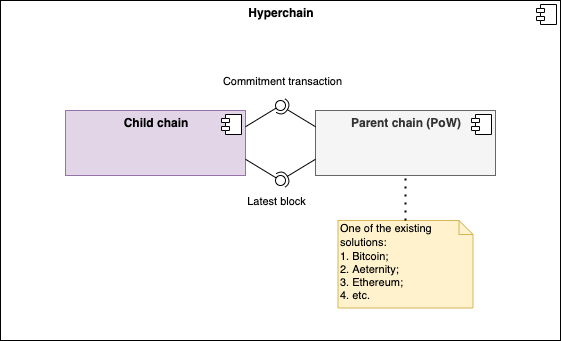
\includegraphics[scale=0.5]{hyperchain_component}
\end{figure}

We define a group of leadership candidates called "delegates." Each delegate
needs to express their will in participation in the election for the upcoming
generation by publishing a commitment transaction onto the parent chain. It is
important to make it clear what is their point of view on the child chain and
over which block they are going to compete.
Therefore the commitment must consist of:
\begin{itemize}
\item The subject of delegation on the child chain
\item The block over the delegate is going to build
\item Signature of the delegate from the child chain
\end{itemize}

One of the important concepts of the commitment idea is to be able to rely on
the parent chain's stability. We want to treat it as a rigid skeleton
of the hyperchain, which can be achieved by proper block hash linking. The
elected leader will be required to publish a key block on the child chain with a
cryptographic proof (referencing the parent) of their right to lead the
upcoming generation and publish microblocks.

One dilemma that rises at this point is whether should the commitment reference
the latest keyblock or the microblock of the child chain. Referencing microblock
on the first sight looks more transparent, but we believe that it would
lead to massive forking (especially when some peers wouldn't receive all of the
blocks). The problem with referencing keyblock is that the next leader could
steal the transactions and post them in their microblocks. This, however, can be
faced with a smarter feeing strategy: instead of giving the full fee to the
miner, we can split it up and give the bigger part to the next leader that did
include the previous leader's microblocks in their continuation of the history,
as it happens in the BitcoinNG\cite{incentive_bcng}.
After getting elected, the new leader posts a keyblock on the child chain that
references the point on the parent, which proves their right to lead the
generation. Besides that, they need to reference the microblock from the previous
generation they want to mine on.


\begin{figure}[h]
	\caption{Hyperchains Design}
	\centering
	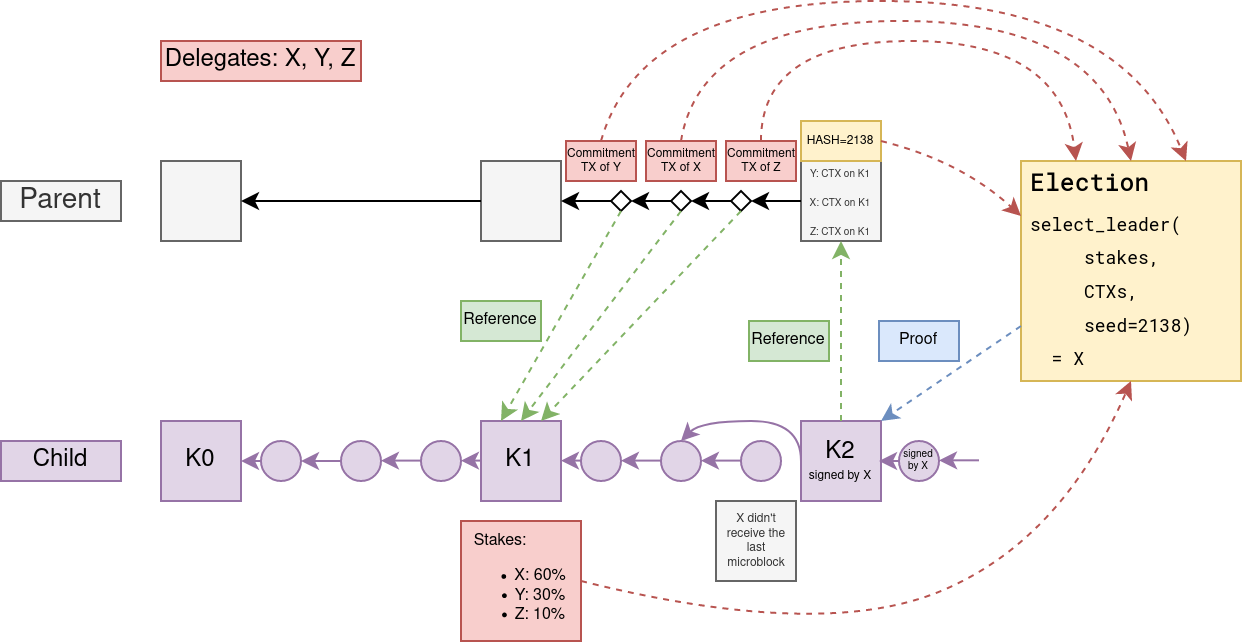
\includegraphics[scale=0.3]{hyperchains_design}
\end{figure}


\section{Election process and staking mechanism}

We do not want to force any particular mechanisms and rules in this section, but
rather propose some solutions that would make it easier to plan and implement
the desired algorithms. This is not up to this document to specify the details.

The most convenient way to organize the election process is to create a smart
contract on the hyperchain that would manage the stake and evaluate PoF
penalties. This contract shall be referenced in the protocol, and its interface
should be settled there. It is eligible for it to be adjusted by regular calls on the fly
– this could save some protocol-level hard forking. If the VM supports it, the
contract could also forcefully alter the blockchain state (i.e., by using some
internal Merkle tree framework). We highly recommend introducing consensus
changes with a decent delay to ensure that it won't break during a true hard fork.

We propose the following features of a staking contract:
\begin{itemize}
\item Leader election
\item Voting power calculation
\item Delegates calculation
\item Voting power delegation
\item Applying punishments
\item Withdrawing and depositing the stake
\item (optional) Controlled hard forking
\end{itemize}

\section{Security}

This hybrid solution allows us to use the parent chain as a reliable protector
against most of the attacks that target the PoS systems\cite{pos_attacks}. In
this section, we assume that the parent chain is well secured, and every user
has stable access to it.

\subsection{Nothing at stake}

This type of attack splits into two cases: micro forks and generational forks.

\subsubsection{Micro forks}

A malicious leader may produce blocks without any cost. They are free to create
conflicting branches within a single generation. This case is very similar to
BitcoinNG's\cite{bcng}. However, this kind of forking is not dangerous in
hyperchains. It may introduce some mess initially but becomes resolved instantly
with the next key block.

\begin{figure}[h]
	\caption{Micro fork}
	\centering
	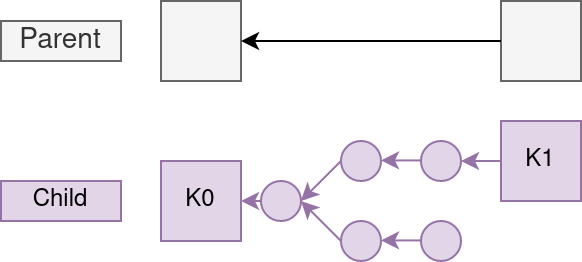
\includegraphics[scale=0.35]{microfork}
\end{figure}

\subsubsection{Generational forks}

This happens when there are multiple key blocks produced by a leader, most
likely as a consequence of a micro fork described above.

\begin{figure}[h]
	\caption{Generational Fork}
	\centering
	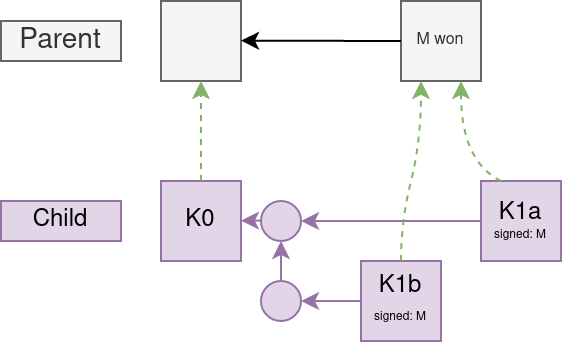
\includegraphics[scale=0.35]{genfork}
\end{figure}

The $K1a$, $K1b$, etc. are key blocks on the child chain emitted by a malicious
leader over different micro blocks. This effectively splits the network, as it
becomes unclear to which of the forks the delegates should commit.

Similarly to PoW chains, this should be solved by the rest of the network.
Eventually some peers should decide on one of the forks, breaking the balance in
the weight function proposed below. After that happens the ``heavier'' chain
shall be deemed the right one. To enforce making a decision, for every candidate
only a single commitment can be counted (most reasonably, the last one in the
parent's block).

A weight function should reflect the total staking power of those who committed
to a fork. The exact logic shall be defined in a smart contract. A simple
example would be the sum of all stakes that were backed by a commitment.

\subsection{Lazy leader}

A leader who does not produce a key block is called ``lazy''. In a case of a
lazy leader, any delegate can produce a key block on behalf of them.
Subsequently, the network is most likely split in the same way as in a
generational fork. Therefore, such a situation shall be resolved the same way.
This also means it makes sense to produce key blocks even while not being a
leader.

In a case in which a lazy leader submits a delayed key block, it is up to the
network whether to consider it. One may argue that a syncing peer would not have
a proof that the leader was ignored due to their laziness, but it is not
different from blacklisting. This behavior is available in almost every PoW and
PoS blockchain and in general does not cause threat, therefore we do not
consider it an issue as well.

\subsection{Stake grinding}

Since the RNG depends exclusively on the key block hash on a PoW chain, it is
impossible to predict its outcomes. One could try to mine the parent chain in a
special way, but it would require so much computational power that in most cases
it would be easier to take control by a 51\% attack.

\subsection{Long range attack}

While it is still possible to perform a long range attack, it would be
impossible to do it secretly and without preparation since the very beginning.
The commitments guarantee that the information of delegates is stored on an
immutable chain, and one would need to announce their will of mining suspicious
blocks during the entire period of the attack. This would quickly expose the
intention of the attacker and let the others prepare for a possible upcoming
attack (by blacklisting them, for example).

\subsection{Overloading parent chain}

Healthy commitment mechanism is key for fair election on a hyperchain. If some
of the delegates get prevented from publishing commitment transactions on the
parent their chances of becoming a leader will vanish regardless of their stake.
This is a vulnerable point of the system. On most blockchains there is a
limitation on the number/total size of transactions in a single block. A
malicious leader could send numerous commitments to fill the entire block
leaving no place for the others.

This strategy hands the staking value to parent's tokens in some sense. The
difference is that in this case the financial effort made to boost one's chances
of being elected is disposable (as long as the attacker did not mine that
block---but then they could just reject other commitments). At the time of
writing the costs of performing such an attack are huge on most blockchains, and
it is almost impossible to sustain it for a longer time. Note that in order to
take full control over just a single generation the attacker would need to
invest funds equal to significantly extended transaction fee multiplied by the
network throughput hoping that every other commitment will get superseded by
\textit{every} of their spam transaction. If it is not enough, performing an
election every $k_{> 1}$th block would greatly amplify the required effort.

\subsection{No commitments}

It may be the case that no one publishes a commitment transaction to a key
block, or that a miner on the parent chain does not include any commitment. We
propose that the smart contract responsible for handling elections should decide
on what happens in that case. For example, a ``lazy leader'' scenario may be
utilized; the previous leader may take over; or the election may be reevaluated
with the candidates from the previous generation.

\section{Derived issues}

While the presented idea seems to cover the majority of cases, some scenarios
may break the system's stability. However, depending on the chosen parent chain
and the tweaks of inner protocol, their impact can be limited to an acceptable
risk.

\subsection{Forks of the parent}

Whatever happens to the parent, the similar shall happen to the child. The child
chain is entirely vulnerable to forks of the parent chain, and it is quite hard
to agree about on which branch to continue. Most likely, the hyperchain would
fork as well. On the other hand, if the validators manage to decide on one
branch, it would be technically possible to jump into the other if the chosen
one becomes less attractive.

\subsection{Attacks on the parent}

The hyperchain can never be more secure than the parent. If somebody succeeds in
a 51\% attack on the parent chain, they will also take control of the child
chain. Therefore the choice of the parent should be made with regards to its
security.

\subsection{Finalization time}

Since there is no single correct strategy on how to react to forks, the
finalization time shall not be shorter on a hyperchain than on the parent chain.
If the parent key block gets rolled back, so will all of the leader elections.

\subsection{Stake collusion}

While stake distribution may look healthy on the surface, stakers can actually
collude rather than act as self-serving actors. As a consequence, there may
emerge a group of delegates whose perceived best interest would be to join a
cartel and unfairly influence the blockchain. This issue, however, is common to
all capital-based PoS systems where power is handed by the value staked in.
Although we do not propose any direct solution to this, a properly tailored
staking contract may address this issue.

\section{Conclusion}

The proposed solution makes it possible to conveniently create simple,
customizable, and most importantly, secure blockchains. The idea of reusing the
existing mining power of other networks allows not only small chains to stay
safe, but also prevents massive energy waste and, therefore, is much more
friendly to the environment. Hyperchains can be utilized in extremely flexible
ways. They can be created and maintained almost for free and in case of network
overload, they can serve as parent chains for other nested child chains. We
leave many implementational details up to the hyperchains creators, because we
find them highly use-case dependent.


\bibliographystyle{acm} \bibliography{bibliography}

\end{document}
